\section{Proponowany podział wybranych metod}
Celem niniejszego przeglądu jest analiza wybranych implementacji stosowanych w wykrywaniu fake newsów. Podzielono je na pięć głównych kategorii: \textbf{modele oparte na drzewach} (Tree-Based Models), \textbf{modele liniowe i statystyczne} (Linear and Statistical Models), \textbf{sieci neuronowe} (Neural Networks), \textbf{zespoły klasyfikatorów} (Ensemble Classifiers) oraz \textbf{modele z ulepszeniami} (Enhanced Models). W każdej z tych kategorii omówiono charakterystyczne cechy oraz innowacyjne modyfikacje w implementacjach, które przyczyniają się do poprawy skuteczności klasyfikacji.


Pragniemy podkreślić, że wszystkie 16 omawianych podejść i implementacji bazują na 16 różnych metodach naukowych, stanowiących fundament analizy. Wybór tych konkretnych metod został podyktowany ich udokumentowaną skutecznością w literaturze naukowej, ze szczególnym uwzględnieniem publikacji z ostatnich lat, które koncentrują się na analizie danych tekstowych i detekcji dezinformacji. Metody te zostały wyselekcjonowane na podstawie ich zdolności do adresowania kluczowych wyzwań w tym obszarze, takich jak przetwarzanie danych, modelowanie złożonych zależności semantycznych oraz radzenie sobie z niezrównoważonymi zbiorami danych, charakterystycznymi dla problematyki fake newsów. Dodatkowo, istotnym czynnikiem wyboru była łatwość implementacji, dostępność propozycji kodu źródłowego w popularnych bibliotekach, gotowych implementacji, oraz programistyczna wygoda, ułatwiająca adaptację i testowanie tych metod w praktyce.


Dodatkowo, proponujemy traktować każde podejście, opisane w jednym z 16 artykułów naukowych, jako odrębną metodę, co ułatwi ich prezentację i wyjaśnienie. Jednocześnie podkreślamy, że autorskie metody, omówione w kolejnych rozdziałach, zostaną przedstawione jako metody numer 17, 18, 19 i 20, uzupełniając cel badania. Autorskie metody różnią się od 16 zaimplementowanych metod opartych na artykułach naukowych tym, że wnoszą oryginalny wkład w analizę i zostały zaimplementowane dzięki głębszemu przejrzeniu 16 różnych metod naukowych.


Ostatnie, ale nie mniej istotne, chcielibyśmy podkreślić, że niektóre metody mogą należeć do kilku możliwych kategorii modeli, ponieważ ich architektura łączy różne techniki klasyfikacyjne, takie jak drzewa decyzyjne i modele zespołowe, co pozwala na elastyczne dostosowanie do specyfiki danych.

\section{Szczegółowy podział wybranych metod}
Niniejszy rozdział prezentuje szczegółowy podział 16 metod klasyfikacyjnych (oznaczonych jako \texttt{metoda1} do \texttt{metoda16}), stosowanych w detekcji dezinformacji, oparty na typie modelu bazowego. Metody podzielono na pięć kategorii: \textbf{modele oparte na drzewach}, \textbf{modele liniowe i statystyczne}, \textbf{sieci neuronowe}, \textbf{zespoły klasyfikatorów} oraz \textbf{modele z ulepszeniami}. Każda metoda jest analizowana pod kątem trzech kluczowych kryteriów: \textbf{zdolności do modelowania złożonych zależności} (nieliniowości w danych tekstowych), \textbf{odporności na niezrównoważenie danych} (istotne w fake newsach, gdzie klasy są często nierównomierne) oraz \textbf{elastyczności preprocessingu} (zdolność do adaptacji do różnych form danych wejściowych,  tekstu czy wektorów TF-IDF). Na poziomie teoretycznym podkreśla się znaczenie tych parametrów, podczas gdy ich strojenie i ostateczne wartości pozostają kwestiami eksperymentalnymi. W każdej metodzie proces klasyfikacji zakłada, że wejściem jest obiekt (wektor cech lub tekst), który przechodzi przez moduł klasyfikacji, a wynikiem jest etykieta binarna określająca grupę przynależności.

\subsection{Modele oparte na drzewach (Tree-Based Models)}
Modele oparte na drzewach wykorzystują drzewa decyzyjne jako fundament klasyfikacji, często ulepszone technikami zespołowymi, takimi jak bagging czy boosting. Dane wejściowe w formie wektora TF-IDF przechodzą przez procesy oparte na drzewach, obejmujące klasyfikację, a potencjalnie preprocessing i post-processing, co prowadzi do wyniku w postaci etykiety binarnej (0/1). Są skuteczne w analizie danych strukturalnych i kategorycznych, co czyni je użytecznymi w detekcji dezinformacji opartej na wektorach cech tekstowych. Proces ten ilustruje diagram przepływu danych \ref{fig:diagram_tree_based_models}, gdzie dane wejściowe (wektor TF-IDF) są przetwarzane przez moduły klasyfikacyjne, takie jak Random Forest, CatBoost czy stacking, a wynikiem jest przypisanie do grupy (etykieta 0/1).

\begin{figure}[H]
	\centering
	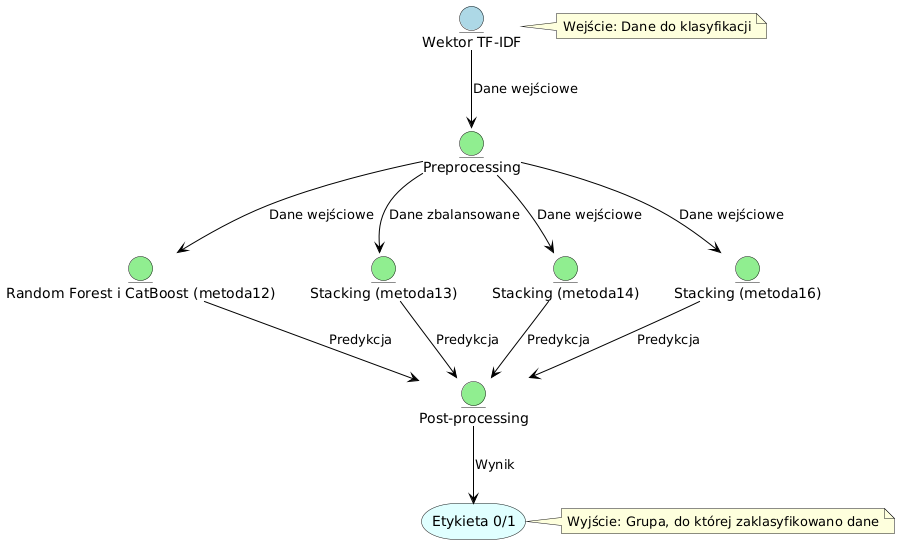
\includegraphics[width=\textwidth]{img/diagrams/Modele oparte na drzewach.png}
	\caption{Diagram przepływu danych dla modeli opartych na drzewach.}
	\label{fig:diagram_tree_based_models}
\end{figure}

Metody oparte na Random Forest obejmują \texttt{metoda7} \cite{metoda7} oraz \texttt{metoda12} \cite{metoda12}. \texttt{Metoda7} łączy Random Forest z Monte Carlo Dropout i heurystycznym post-processingiem, oferując następujące parametry:
\begin{itemize}
    \item n\_samples = 50 – Określa liczbę próbek w Monte Carlo Dropout, co pozwala szacować niepewność predykcji i zwiększa odporność na niezrównoważenie danych.
    \item n\_estimators = 100 – Liczba drzew w Random Forest, wpływa na dokładność i stabilność klasyfikacji poprzez zwiększenie różnorodności modelu.
    \item threshold = 0.9 – Próg w heurystycznym post-processingu, decyduje o korekcie predykcji na podstawie meta-danych, wiarygodności źródła.
\end{itemize}
Proces ten przedstawia diagram aktywności w notacji UML, który pokazuje sekwencję kroków oraz decyzje, jak zilustrowano w diagramie \ref{fig:diagram_aktywnosci_metoda7}. Również przyjrzyjmy się procesowi klasyfikacji z perspektywy diagramu blokowego, który przedstawia ciąg etapów w uczeniu maszynowym, jak ukazano w diagramie \ref{fig:diagram_blokowy_metoda7}.

\begin{figure}[H]
    \centering
    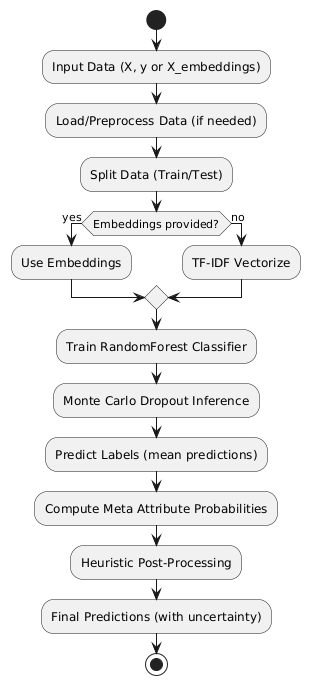
\includegraphics[height=0.4\textheight]{img/diagrams/Diagram Aktywności metoda 7.png}
    \caption{Diagram aktywności dla metody 7.}
    \label{fig:diagram_aktywnosci_metoda7}
\end{figure}

\begin{figure}[H]
    \centering
    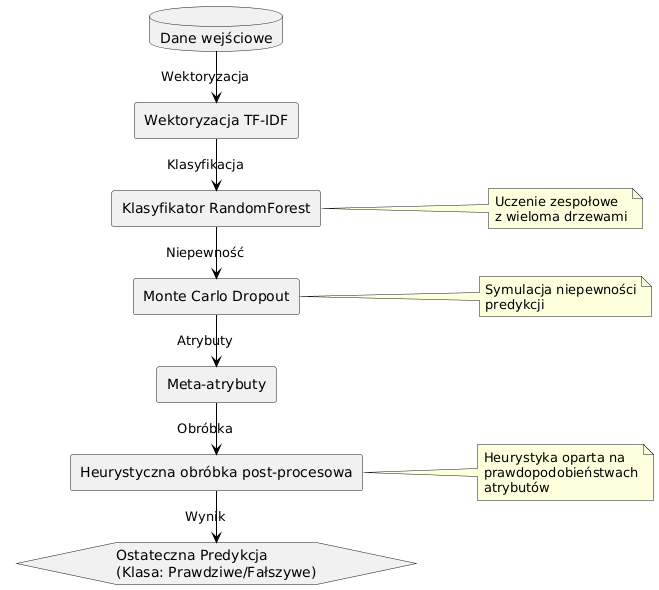
\includegraphics[width=0.9\textwidth]{img/diagrams/Diagram blokowy metoda 7.png}
    \caption{Diagram blokowy dla metody 7.}
    \label{fig:diagram_blokowy_metoda7}
\end{figure}

% Z kolei \texttt{metoda12} porównuje Random Forest z CatBoost, z parametrami:
% \begin{itemize}
% 	\item n\_estimators = 100 – Liczba drzew w Random Forest, kluczowa dla modelowania złożonych wzorców tekstowych.
% 	\item iterations = 200 – Liczba iteracji w CatBoost, określa głębokość uczenia się boostingowego, co poprawia zdolność do analizy nieliniowości.
% 	\item learning\_rate = 0.01 – Tempo uczenia w CatBoost, reguluje kompromis między dokładnością a szybkością treningu, istotny dla elastyczności preprocessingu.
% \end{itemize}
% Proces ten przedstawia diagram UML, który opisuje i pokazuje przepływ klasyfikacji. \texttt{Metoda7} wyróżnia się odpornością na niezrównoważenie dzięki analizie niepewności, podczas gdy \texttt{metoda12} oferuje elastyczność w preprocessingu danych kategorycznych poprzez CatBoost.

% W stackingach drzewiastych znajdziemy \texttt{metoda13} \cite{metoda13}, \texttt{metoda14} \cite{metoda14} i \texttt{metoda16} \cite{metoda16}. \texttt{Metoda13} wykorzystuje Random Forest, Gradient Boosting i XGBoost z parametrami:
% \begin{itemize}
% 	\item n\_estimators = 100 – Liczba drzew w każdym modelu, zwiększa zdolność do modelowania złożonych zależności w danych.
% 	\item learning\_rate = 0.1 – Tempo uczenia w XGBoost i Gradient Boosting, wpływa na precyzję boostingowego uczenia się.
% 	\item SMOTETomek – Strategia balansowania klas, poprawia odporność na niezrównoważenie poprzez nad- i podpróbkowanie.
% \end{itemize}
% Proces ten przedstawia diagram UML, który opisuje i pokazuje przepływ klasyfikacji.

% \texttt{Metoda14} opiera się na Random Forest i AdaBoost:
% \begin{itemize}
% 	\item n\_estimators = 100 – Liczba drzew w Random Forest i AdaBoost, kluczowa dla stabilności i dokładności.
% 	\item learning\_rate = 0.5 – Tempo uczenia w AdaBoost, reguluje wagę błędnie sklasyfikowanych przykładów, co zwiększa odporność na nierównowagę.
% \end{itemize}
% Proces ten przedstawia diagram UML, który opisuje i pokazuje przepływ klasyfikacji.

% \texttt{Metoda16} stosuje Random Forest i Gradient Boosting:
% \begin{itemize}
% 	\item n\_estimators = 100 – Liczba drzew, determinuje zdolność do wychwytywania złożonych wzorców.
% 	\item learning\_rate = 0.1 – Tempo uczenia w Gradient Boosting, wpływa na dokładność modelu w iteracyjnym uczeniu.
% \end{itemize}
% Proces ten przedstawia diagram UML, który opisuje i pokazuje przepływ klasyfikacji. Te metody łączą siłę drzew w modelowaniu danych tekstowych, a SMOTETomek w \texttt{metoda13} dodatkowo zwiększa odporność na niezrównoważenie.

% \subsection{Modele liniowe i statystyczne}
% Modele liniowe i statystyczne opierają się na liniowych lub statystycznych regułach decyzji, oferując interpretowalność. Obiekt,  wektor cech, jest klasyfikowany przez moduł liniowy lub statystyczny, dając etykietę binarną.
% Ta kategoria obejmuje modele wykorzystujące liniowe granice decyzji lub reguły statystyczne, takie jak regresja logistyczna czy SVM. Ich zaletą jest interpretowalność i efektywność w prostszych zbiorach danych. Modyfikacje, takie jak regularyzacja w regresji logistycznej, pomagają dostosować je do bardziej złożonych problemów.


% Metody z regresją logistyczną jako meta-modelem to \texttt{metoda2} \cite{metoda2} (Gradient Boosting i MLP), \texttt{metoda5} \cite{metoda5} (Random Forest i XGBoost) i \texttt{metoda16} \cite{metoda16} (Random Forest, Gradient Boosting, SVM), z parametrem max\_iter ( 1000) kluczowym dla konwergencji. Ich elastyczność preprocessingu jest ograniczona, ale dobrze radzą sobie z prostymi danymi. 

% W votingach statystycznych \texttt{metoda3} \cite{metoda3} (SVM z C = 1.0, Naive Bayes z alpha = 0.5), \texttt{metoda9} \cite{metoda9} (Logistic Regression, SVM) i \texttt{metoda11} \cite{metoda11} (Logistic Regression) oferują prostotę i odporność na niezrównoważenie dzięki konsensusowi, choć słabiej modelują nieliniowości.

% \subsection{Sieci neuronowe}
% Sieci neuronowe modelują złożone zależności w danych tekstowych i sekwencyjnych. Obiekt,  tekst lub sekwencja, przechodzi przez moduł neuronowy, dając etykietę binarną.
% Sieci neuronowe wyróżniają się zdolnością do modelowania nieliniowych zależności w danych sekwencyjnych i tekstowych. Wykorzystują warstwy neuronowe, takie jak LSTM czy CNN, do analizy skomplikowanych wzorców. Innowacyjne podejścia,  hybrydowe połączenie Bi-LSTM i CNN, zwiększają ich skuteczność w zadaniach wymagających głębokiego przetwarzania danych.

% Głębokie sieci to \texttt{metoda1} \cite{metoda1} (Dense z units = 128/64/32, dropout\_rate = 0.2), \texttt{metoda4} \cite{metoda4} (Bi-LSTM z 128 jednostkami, CNN z kernel\_size = 5) i \texttt{metoda15} \cite{metoda15} (Bi-LSTM z embedding\_dim = 200). Parametry jak liczba jednostek czy dropout zwiększają zdolność do modelowania nieliniowości i elastyczność preprocessingu ( tokenizacja). \texttt{metoda10} \cite{metoda10} używa MLP (hidden\_layer\_sizes = 14) w voting, oferując prostszą neuronową analizę.

% \subsection{Zespoły klasyfikatorów}
% Zespoły klasyfikatorów integrują różne modele via stacking lub voting. Obiekt,  wektor cech, jest klasyfikowany przez moduł zespołowy, dając etykietę binarną.
% Metody te integrują różne klasyfikatory poprzez techniki stacking lub voting, łącząc ich mocne strony dla lepszej dokładności. Modyfikacje, takie jak dwupoziomowe voting czy użycie meta-modeli, pozwalają na elastyczne dostosowanie do specyficznych problemów.

% Stackingi to \texttt{metoda2} \cite{metoda2}, \texttt{metoda5} \cite{metoda5}, \texttt{metoda13} \cite{metoda13}, \texttt{metoda14} \cite{metoda14} i \texttt{metoda16} \cite{metoda16}, z kluczowymi parametrami jak n\_estimators czy max\_iter w meta-modelach. Votingi to \texttt{metoda3} \cite{metoda3}, \texttt{metoda6} \cite{metoda6} (z BERT batch\_size = 32), \texttt{metoda8} \cite{metoda8}, \texttt{metoda9} \cite{metoda9}, \texttt{metoda10} \cite{metoda10} i \texttt{metoda11} \cite{metoda11}. Elastyczność preprocessingu ( Chi-kwadrat w \texttt{metoda11}) i modelowanie złożoności są tu silne, a SMOTETomek w \texttt{metoda13} wspiera niezrównoważenie.

% \subsection{Modele z ulepszeniami}
% Modele z ulepszeniami dodają techniki korygujące. Obiekt,  TF-IDF, przechodzi przez moduł z ulepszeniami, dając etykietę binarną.
% Modele te rozszerzają standardową klasyfikację o dodatkowe techniki, takie jak post-processing czy analiza niepewności. Innowacje, takie jak Monte Carlo Dropout i heurystyczne korekty, poprawiają jakość predykcji, zwłaszcza w trudnych przypadkach.

% \texttt{metoda7} \cite{metoda7} (Random Forest z Monte Carlo Dropout, num\_samples = 50) stosuje heurystykę, co zwiększa precyzję w modelowaniu złożonych danych tekstowych i odporność na niezrównoważenie poprzez analizę niepewności.